\section{Related Work}

\subsection{Tasking}
\label{subsec:Tasking}
  Having the task construct as mean to parallelize a program allows to utilize irregular parallelism.
  Irregular parallelism is widely used these days and includes parallel execution of while loops or recursive function calls for instance.
  Tasking explicitly specifies independent units of work which can be executed in parallel.
  This enables a more dynamic way of parallelization.
  However, a disadvantage of this kind of parallelism is that it increases the complexity of a program and poor implementations can lead to an increased overhead.~\cite{Ayguade.2009}~\cite{LaGrone.2011}
  
  
  The used runtime system plays a crucial role when it comes to the application's performance using tasking. 
  For example, as the tasking construct creates several tasks which will be executed by threads, the performance of an application relies on the thread scheduler of the runtime system.
  The authors of \cite{LaGrone.2011} discuss different aspects of a runtime system using the task construct.
  The efficiency of such depends on the data structures which store unfinished tasks, manage task switching and regulate task creation.
  Additionally, the data structures to organize task synchronization and manage the memory footprint of a task are also important.
  The ideal way of work of the thread scheduler, for example, is to maximize concurrency, load balancing and data locality.
  This can be achieved by different ways to manage queue storing all tasks ready to be executed.
  Furthermore, the scheduler can be \textit{depth-first} or \textit{breadth-first}.
  Breadth-first means that child tasks created by the parent task and put into the queue to be scheduled at any time.
  Whereas breadth-first schedulers switch to child tasks directly after their creation and execute them.
  This leads to a smaller number of tasks in the queue and less concurrency opportunities.
  However, the data reuse increases.
 
 	
  The following subsections \ref{subsec:OpenMP} and \ref{subsec:HPX} introduce two runtime systems utilizing tasks.
  These will be compared in this work.


\subsection{Tasks in OpenMP}
\label{subsec:OpenMP}
  OpenMP includes the tasking model since version 3.0.
  Various directives for that purpose are being included since to specify and manage  tasks.
  However, OpenMP still differs between explicit and implicit tasks.
  Implicit tasks are created by parallel regions as side effect.
  The programmer does not need to specify or know about them.
  Explicit tasks on the other hand are defined by the programmer using the task directives.
  The simplest directive to define an explicit task is \texttt{omp task} and the enclosed code area is the task region.
  These are executed by any task in the current team whenever they are ready.~\cite{Ayguade.2009}~\cite{LaGrone.2011}

%MAYBE example implementation here - show the directives

  When a thread encounters a task directive the current data environment is captured.
  This environment and the block of code in the task region form the generated task.
  The variable scopes of a task region can be defined like in parallel regions.
  By adding the clauses \texttt{shared}, \texttt{private} or \texttt{firstprivate} to the task directive the declared variables are either shared among tasks or not.~\cite{Duran.2008}
  
  
  By default a thread is tied to a task as it begins to execute it.
  This means that this task is only allowed to be executed by one thread.
  However this thread can still execute other tasks in case it reaches task scheduling points and switches the execution to another task.
  The suspended task is put into the queue and has to wait until its tied thread is ready to continue its execution.
  This restriction can be avoided by defining the task \texttt{untied}.
  By doing so, load balancing is increased, but data locality is decreased.~\cite{Ayguade.2009}~\cite{LaGrone.2011}


  Tasking results in a more dynamic execution and might be unpredictable without explicit scheduling.
  For example the runtime system has either a depth- or breadth-first scheduler.
  Meaning that it either switches to the child task after creation or finishes the parent task first.
  The used OpenMP runtime system is responsible to decide.
  Explicit scheduling can be used to avoid this uncertainty.
  For instance, adding an \texttt{if}-clause to the task directive and evaluating it to false makes the encountering thread to suspend its current work and execute the child task immediately.
  Furthermore, explicit task scheduling is possible by using the \texttt{taskwait} and \texttt{barrier} directives.
  \texttt{taskwait} suspends the encountering task region and forces it to wait for all child tasks to complete.
  Additionally \texttt{taskgroup} defines a task region which will be executed and at the end the current task has to wait for all its child and their descendants.~\cite{Qawasmeh.2014}~\cite{Furlinger.2009}


\subsection{HPX}
\label{subsec:HPX}
\subsubsection{HPX}
  %1\cite{Kaiser.2014}
  %2\cite{Kaiser.2009}	  
  
  HPX aims to resolve problems in scalabilitiy, power efficiency, resource management and even further ones which may raise and increase by moving from Peta- to Exascale systems.
  It focuses on parallel and distributed development independent of the system's scale.
  This is done by providing a general purpose C++ runtime system with an innovative design.
  It is described as a mixture of lightweight synchronization, global system-wide address space and fine grain parallelism.
  Message driven computation can be achieved with a small amount of effort.
  A remote execution has the same semantics as a local one and can thereby be done implicitly.
  Furthermore, it offers the programmer explicit support for accelerators such as general purpose graphical processing units.~\cite{Kaiser.2014}
  
  
  A new model of parallel execution is introduced to enable all of this features --- called \textit{Parallex}.
  HPX is the runtime system supporting this new model.
  It consists of components which can be seen in figure \ref{fig:HPXcomp}.
  Additionally, it shows the current architecture of HPX and how the following ParalleX components are included.~\cite{Kaiser.2009}\\
  \textbf{Parcel Subsystem} encapsulates method calls into parcels.
  These contain the global address of the object whose method is called and the necessary arguments.
  Parcels are communicated via localities which are placed on each node and can be seen as parcel interfaces.
  The parcel subsystem is especially useful when it comes to remote method calls.\\
  \textbf{Active Global Address Space (AGAS)} includes all localities the current application is using.
  Global identifiers ease to locate objects in the network.
  Having this global address space furthermore allows to move objects across localities without changing its address.\\  
  \textbf{Instrumentation and Adaptivity} includes several performance countering and monitoring tools.
  They might be helpful when debugging or analyzing the program and offer insights without using additional tools.\\
  \textbf{Threading Subsystem} uses a work-queue based execution strategy to schedule HPX threads.
  These are either created locally or the threading subsystem converts parcels on receive into HPX threads.
  In contrast to other systems the ParalleX model maps \(m\) internal threads instead of just 1 onto \(n\) kernel threads.
  This allows ParalleX to switch between threads without the need of kernel calls and their context switch overhead.\\  
  \textbf{Local Control Objects (LCO)} are used for scheduling and abstract mechanism used to do so.
  For example, \textit{futures} are proxies for results not yet known and can only be accessed after the result is available.
  In case the future is accessed earlier, the thread doing so is suspended.
  Additional to special objects such as futures, HPX also offers traditional concurrency control mechanisms, for instance mutexes and semaphores.
\begin{figure}[htbp]
	\centering
	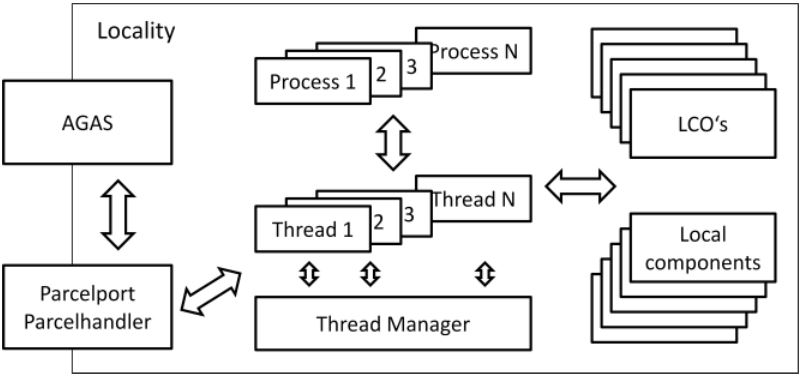
\includegraphics[width=0.45\textwidth]{figures/parallexArchitecture.JPG}
	\caption{ParalleX Components Implemented in HPX~\cite{Kaiser.2009}}
	\label{fig:HPXcomp}
\end{figure}
  	
	
\subsubsection{Tasks in HPX}
  \label{subsubsec:TasksHPX}
  Various program models increase their efforts on tasking in recent years and increase the possibilities in local parallelism.
  However, in contrast to the other program models, HPX offers a way for homogeneous execution of local and remote operations.
  This is achieved by using the task model combined with a so called \textit{Active Global Address Space}.
  As all nodes of an application share a common address space, objects and tasks can be migrated across nodes.
  Instead of moving the data to nodes the tasks can be moved to the data, which allows faster communication as the instructions are often smaller in size than the actual data.
  Furthermore the migration can be done without changing the global address as all nodes share the address space.
  Additional work is saved due to this fact.~\cite{Kaiser.2014}
  
  Another advantage of HPX which also makes it convenient to C++/C programmers is that it uses the same tasking methods as the C++ standard.
  No new semantic or syntax is used.
  However, the actual standard is extended to support remote operations.
  To use tasking in HPX, tasks have to be defined by \texttt{async} and \texttt{future}.
  \texttt{async} launches a task asynchronously.
  \texttt{future<T>} represents a value of type \texttt{T} which will be available in the future, when the execution of a task finishes.
  It acts as a placeholder of a result not known yet and when created spawns a new HPX-Thread which is placed on the thread queue.
  In case another thread wants to access a future it is blocked and has to wait until the value of the future is available.
  Using \texttt{get()} is an explicit option for the programmer to let the thread wait for the future.~\cite{Kaiser.2014}~\cite{TheSTEARGroup.2020}
  
  
  The HPX thread scheduling system uses lightweight threads which allow faster context switches and smaller stacks.
  Task migration is therefore more efficient as less data has to be moved.
  Furthermore, it is designed to handle millions of tasks efficiently.
  In \cite{Kaiser.2014} HPX tasks are compared to OpenMP tasks for their GFLOPS on various numbers of cores.
  However the HTTS benchmark is used which uses no-op tasks and can therefore only compare the thread scheduling performance without actual workload.
  One reason why HPX performed better in the HTTS benchmark is that it uses constraint based synchronization instead of global barriers, like in OpenMP.
  For example, OpenMP uses implicit barriers at the end of each loop.
  In contrast to that HPX allows to execute the code following the loop in case no data dependencies are given.
  
     
\subsection{Benchmark Algorithms}
\label{subsec:BOTS}
  The authors of \cite{Duran.2009} introduce a benchmark suite to test the impact of different implementation decisions using OpenMP tasks.
  The benchmark suite is called \textit{Barcelona OpenMP Task Suite (BOTS)} and includes nine benchmarks:\\
    \textbf{Alignment} is an algorithm aligning protein sequences against every other sequence.\\
    \textbf{Fourier Transformation} tries to approximate a periodic function by several subfunctions.\\
    \textbf{Fibonacci} calculates the \(n^{th}\) number of the Fibonacci sequence.\\
    \textbf{Floorplan} computes the optimal floorplan distribution of a number of cells.\\
    \textbf{Health} simulates the Colombian Health Care System.\\
    \textbf{N Queens} tries to find placements of \(n\) queens on a chessboard under special condition.\\
    \textbf{Sort} is a special kind of parallel merge sort execution.\\
    \textbf{SparseLU} calculates a LU matrix factorization over sparse matrices.\\
    \textbf{Strassen} hierarchically decomposes a matrix for multiplication of large dense matrices.\\
  The suite offers different versions of each benchmark, e.g. a version of Fibonacci using a cut-off to avoid an high amount of tasks.
 
 
\subsection{hpxMP}
  A rather new approach is \textit{hpxMP}.
  It's an implementation of the OpenMP standard using an underlying hpx system and introduced in \cite{hpxMP.2019}.
  The motivation of this approach is to ease the migration from OpenMP to Asynchronous Many-Task (AMT) systems.
  AMT as a new parallel programming paradigm utilizes fine grained tasks to distribute the workload across multiple node.
  It is similar to the well known \textit{MPI+X} approach in which the Message Passing Interface (MPI) is used together with OpenMP for example.
  However, MPI+X lacks scalability and parallel efficiency compared to AMTs.
  HPX as an example for an AMT might also be more convenient as it follows the newest C++ standard and therefore has a more flatten learning curve for C++ programmers.
  Another advantage of hpxMP might have in contrast to MPI+X is that it uses HPX lightweight threads instead of system threads.
  They are briefly explained in \ref{subsubsec:TasksHPX}.
  
  \begin{figure}[htbp]
	\centering
	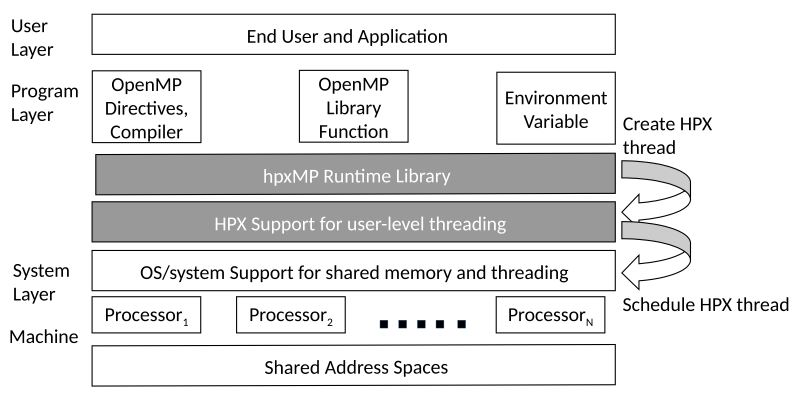
\includegraphics[width=0.48\textwidth]{figures/hpxMP.JPG}
	\caption{Adaption of an OpenMP Application to use hpxMP~\cite{hpxMP.2019}}
	\label{fig:hpxMP}
  \end{figure}
  
  Figure \ref{fig:hpxMP} shows how hpxMP can be used to run OpenMP applications.
  The application is compiled with OpenMP flags, but linked against the hpxMP runtime library being the first grey layer in the figure.
  Instead of calling the OpenMP functions, equivalent hpxMP functions are called.
  These redirect the calls to appropriate functions of the underlying HPX system being the next grey layer in the figure.
  This system allows to execute OpenMP applications using HPX according to the OpenMP standard.
  
  The authors of \cite{Zhang.2192020} furthermore extended hpxMP with further task features of the OpenMP 5.0 standard.
  Additionally, they compared the new hpxMP system with different OpenMP implementations.
  Among other benchmarks, they used the BOTS merge sort algorithm.
  The cut off option is used to decrease the number of tasks spawned.
  The results show that hpxMP can already reach similar or better performance results for larger input sizes.
  This is due to the fact that joining a large number of tasks after a parallel region produce less overhead using HPX threads.
  Compared to conventional operating system threads HPX threads are lightweight and need less effort when joining.
  However for smaller input sizes hpxMP reaches slower performance.
  The authors explain this by the overhead which is introduced by the HPX scheduler.
  Conventional threads spawned by OpenMP may not be suspended and therefore need to be scheduled less often.
  